\chapter{MARCO TEÓRICO}

\section{Antecedentes del Problema}

\subsection{Antecedentes internacionales}
En el contexto de la sostenibilidad ecológica y la gestión ambiental, el estudio titulado \textit{``Water Quality Assessment of Laguna de Bay Through Geostatistical Analysis of Physicochemical Parameters''} proporciona un análisis detallado y crítico de la calidad del agua en Laguna de Bay. A través de una modelización geoestadística que incorpora parámetros fisicoquímicos, el estudio evidencia la preocupante tendencia de deterioro de la calidad del agua y la salud del ecosistema del lago, afectado significativamente por las prácticas acuícolas y la inadecuada eliminación de residuos \cite{Bernal2022}. La actualización de este modelo geoestadístico para octubre de 2020, incluyendo variables como la demanda biológica de oxígeno, oxígeno disuelto, pH, amoníaco, nitrato y fosfato inorgánico, es una herramienta esencial que verifica la efectividad de las estrategias de desarrollo sostenible adoptadas y resalta la continua necesidad de monitoreo y acción para preservar la integridad del lago. Este enfoque metodológico subraya la utilidad de los modelos geoestadísticos en la evaluación y monitorización de los sistemas lacustres, incluso con datos limitados, y sugiere la incorporación de información adicional para refinar y mejorar la precisión de estos modelos. 

En el estudio titulado \textit{``A geostatistical approach to optimize water quality monitoring networks in large lakes: Application to Lake Winnipeg''}, se aborda el monitoreo de la calidad del agua en grandes lagos, enfocándose en el diseño óptimo de redes de monitoreo mediante métodos geoestadísticos \cite{Beveridge2012}. El estudio resalta la importancia de la ubicación de las estaciones de muestreo en la red de monitoreo, un componente crítico para la recogida eficaz de datos. Utilizando el Lago Winnipeg en Canadá como caso de estudio, se colectaron muestras de isótopos de agua ($\delta$2H, $\delta$18O) en aproximadamente 240 estaciones a lo largo del lago. La investigación empleó dos enfoques estadísticos para evaluar la redundancia en esta densa red de muestreo: el kriging, una técnica de interpolación espacial, y los valores de Moran's I local. El kriging se utilizó para evaluar la idoneidad de la configuración de la red muestreada, mientras que Moran's I identificó agrupaciones de estaciones similares o diferentes.

La aplicación de estos métodos reveló que, aunque individualmente muchas estaciones podrían considerarse redundantes, la redundancia dependía de la premisa de que todas las demás estaciones permanecieran en la red. Al analizar agrupaciones de estaciones, se determinó que hasta cuatro estaciones podrían eliminarse de cada grupo sin una pérdida significativa de información. Este hallazgo fue confirmado por los valores de Moran's I local \cite{Beveridge2012}. Este enfoque integral permitió identificar estaciones que eran estadísticamente importantes o redundantes dentro de la red. El estudio subraya la relevancia de evaluar la información proporcionada por una estación individual en el contexto de un grupo de estaciones dentro de una red. La metodología propuesta en este estudio, que combina kriging y Moran's I, podría aplicarse ampliamente para la validación objetiva de redes de monitoreo de la calidad del agua en lagos, abarcando una variedad de parámetros de interés como nutrientes y contaminantes.

En el artículo \textit{``An Application of Geostatistics to Analysis of Water Quality Parameters in Rivers and Streams in Niger State, Nigeria''}, se explora la importancia de incorporar la localización espacial en la evaluación de la calidad del agua superficial, destacando cómo la variabilidad espacial puede ayudar a identificar el grado de contaminación por escorrentía y actividades antropogénicas \cite{Audu2015}. Utilizando técnicas geoestadísticas y una variedad de paquetes de software, el estudio se enfoca en cinco parámetros de calidad del agua en varios ríos y arroyos del estado de Níger en Nigeria. Se generaron variogramas y mapas espaciales krigeados para las estaciones de lluvia y seca, revelando una alta coherencia espacial para parámetros como E.coli, Mg y Sólidos Totales Disueltos (TDS), mientras que otros mostraron menor coherencia.

Este análisis detallado proporciona una comprensión más profunda de las dinámicas de calidad del agua en la región, resaltando la utilidad de las técnicas geoestadísticas en la gestión de recursos hídricos. El contexto de Níger State, con sus dos estaciones climáticas distintas, resalta la variabilidad en la disponibilidad y calidad del agua, exacerbada por el aumento de la población y la demanda de agua potable \cite{Audu2015}. Esta variabilidad estacional afecta no solo a la disponibilidad de agua sino también a sus características fisicoquímicas y microbiológicas, lo que hace esencial el monitoreo durante todo el año. La combinación de herramientas estadísticas multivariadas y técnicas geoestadísticas utilizadas en este estudio muestra cómo se pueden identificar fuentes potenciales de contaminación del agua y proporcionar una base sólida para una gestión eficaz y sostenible de los recursos hídricos. La metodología aplicada en este estudio ofrece un modelo valioso para la validación objetiva de las redes de monitoreo de la calidad del agua y resalta la creciente importancia de enfoques integrados para abordar problemas ambientales complejos.

En el estudio \textit{``Evaluating the effectiveness of routine water quality monitoring in Miyun reservoir based on geostatistical analysis''}, se emplean técnicas de sistemas de información geográfica y métodos geoestadísticos para evaluar la eficacia del monitoreo rutinario de la calidad del agua en el segmento occidental del embalse de Miyun en Beijing \cite{Zhengjun2010}. El estudio se centra en evaluar tanto las metodologías como el diseño de muestreo empleados en el monitoreo. Se utilizan métodos de evaluación tanto de capa única como métodos integrados, incluyendo análisis de componentes principales (PCA), kriging ordinario (OK)\_Media, y Media\_Capas, para validar la efectividad de los métodos de evaluación.

Los resultados revelan que mientras la evaluación de capa única solo muestra el estado trófico del agua en un nivel específico, una evaluación integrada analiza y evalúa de manera sintética el estado trófico de todo el cuerpo de agua. Los resultados del análisis integrado indican que el método PCA es más preciso y representa mejor el estado trófico de todo el cuerpo de agua. Por otro lado, los métodos OK\_Media y Media\_Capas solo logran representar el nivel medio del estado trófico de todo el cuerpo de agua, pero no reflejan el estado trófico local ni los detalles de la distribución \cite{Zhengjun2010}. A pesar de que los métodos utilizados en el monitoreo rutinario del embalse de Miyun tienen algunas similitudes con los métodos OK\_Media y Media\_Capas, el rango de errores y la incertidumbre son mayores debido a la falta de información espacial continua detallada.

Además, el análisis sobre el número de puntos de muestreo muestra que, dentro de un cierto rango de error, cambios menores en los puntos de muestreo no tendrán un impacto significativo en los resultados del monitoreo. Para el monitoreo rutinario del segmento occidental del embalse de Miyun, el uso de solo tres a cinco puntos de muestreo resulta insuficiente. Según el análisis, es más apropiado utilizar al menos diez puntos de muestreo para monitorear estas áreas \cite{Zhengjun2010}.



En el estudio \textit{``Characterizing, predicting, and mapping of soil spatial variability in Gharb El-Mawhoub area of Dakhla Oasis using geostatistics and GIS approaches''}, el objetivo principal es determinar, predecir, mapear y evaluar la variabilidad espacial de los atributos fisicoquímicos del suelo utilizando técnicas de sistemas de información geográfica (GIS) y métodos geoestadísticos. Se enfoca en 34 perfiles de suelo geo-referenciados en el área de Gharb El-Mawhoub de Dakhla Oasis, analizando una gama de propiedades fisicoquímicas del suelo como la conductividad eléctrica, la textura, y otros elementos como carbonato de calcio y materia orgánica. Para llevar a cabo el análisis, el estudio empleó modelos semi-variogramas para cuantificar la variación espacial y la técnica de kriging ordinario para generar mapas correspondientes. Además, se realizaron pruebas de validación cruzada para evaluar la precisión de los modelos predictivos. Los resultados destacaron diferencias considerables en las características del suelo a lo largo de la región estudiada, con coeficientes de correlación significativos. Además, se identificaron modelos semi-variogramas específicos como los más adecuados para las propiedades del suelo investigadas, y los mapas predictivos generados ofrecen información valiosa para la agricultura de precisión, mejorando la productividad del suelo y reduciendo limitaciones. Estos hallazgos demuestran que los enfoques geoestadísticos son técnicas poderosas para determinar, predecir y mapear las interrelaciones espaciales de los atributos del suelo, esenciales para la gestión específica del sitio y la promoción del desarrollo sostenible en áreas agrícolas.\cite{Selmy2022}.

El estudio titulado \textit{``Mapeamento da distribuição espacial da qualidade da água em função do uso e da ocupação do solo e da precipitação na Bacia do Rio Pará, MG''} se enfocó en mapear la distribución espacial de la calidad del agua, la precipitación y el uso y ocupación del suelo en la Bacia Hidrográfica del Rio Pará utilizando técnicas de geoestadística \cite{sousa}. El objetivo principal era comprender cómo la variabilidad espacial de los parámetros fisicoquímicos del agua podría relacionarse con el uso del suelo y la precipitación, impactando en el planeamiento y manejo de la bacia. 

Metodológicamente, el estudio utilizó datos de calidad y precipitación muestreados en 25 puntos entre 1997 y 2018, aplicando el test de coeficiente de Pearson y generando mapas de kriging ordinaria para aquellos parámetros que mostraron fuertes correlaciones. Además, se elaboraron mapas de uso y ocupación del suelo para proporcionar una visión integral del área de estudio\cite{sousa}.

Los resultados revelaron diferencias significativas en la distribución de la precipitación entre períodos secos y lluviosos, y los análisis indicaron una correlación entre los niveles elevados de variables como nitrógeno, fósforo, coliformes termotolerantes, y otros, con áreas urbanas dentro de la cuenca. Este estudio no solo subraya la importancia del monitoreo de la calidad del agua en la gestión de recursos hídricos sino también demuestra la utilidad de la geoestadística como una herramienta poderosa para entender la interacción entre el agua, el suelo y el uso humano del paisaje \cite{sousa}.

\subsection{Antecedentes Nacionales}
En el humedal laguna Los Milagros, ubicado a 25 km de la ciudad de Tingo María en el departamento de Huánuco, se realizó una investigacion obtuvo ión para determinar la calidad del agua utilizando el Índice de Calidad del Agua de la National Sanitation Foundation de Estados Unidos (NSF). Se evaluaron parámetros fisicoquímicos como oxígeno disuelto, demanda bioquímica de oxígeno, sólidos totales disueltos, turbidez, pH, temperatura, nitratos, fosfatos totales y coliformes fecales. Se recolectaron muestras en cuatro estaciones de muestreo establecidas en la laguna, y luego se procesaron los datos para calcular el Índice de Calidad del Agua, que un valor de 62, correspondiente a una calidad media. Se concluyó que la laguna se ve afectada durante el período de estiaje debido a la entrada de aguas contaminadas, el uso de fertilizantes en áreas cercanas, actividades de pastoreo de ganado y la instalación de letrinas, lo que afecta la conservación del ambiente acuático y su utilización \cite{alarcon}.

Se realizo una investigacion titulada \textit{``Evaluación de la calidad del agua del río Rímac mediante el análisis multivariado ``} el cual se centró en la aplicación de técnicas estadísticas multivariadas para evaluar y clasificar espacialmente los datos obtenidos durante el monitoreo del agua en la cuenca seca, parte de la cuenca húmeda y el principal tributario del río Rímac, el río Santa Eulalia, en el departamento de Lima. Se recolectaron 252 muestras de agua en 7 estaciones de muestreo a lo largo del río y su tributario, analizando 20 parámetros físicos y químicos en cada una. Se utilizaron técnicas de análisis de clúster, análisis de componentes principales, análisis de factor y análisis discriminante para evaluar y clasificar los datos. Estas técnicas permitieron agrupar las estaciones de muestreo y los parámetros ambientales en diferentes clases, lo que ayudó a identificar 4 fuentes principales de contaminación que influyen en la composición del agua del río \cite{Espiritu2010}.

En la investigación intitulada \textit{``Evaluación de Impacto Ambiental en el Santuario Nacional de Ampay - Apurímac''}, se observó que la laguna Ankasqocha presenta un proceso de eutrofización mayor que la laguna Usphaqocha. Las aguas contenidas en el reservorio del Santuario, utilizadas con fines agrícolas, están clasificadas como agua de salinidad media, apta para riego. Se encontró que las lagunas Ankasqocha y Usphaqocha presentan niveles bajos de nitratos, fosfatos, cloruros y sulfatos. En particular, la laguna Ankasqocha evidencia un proceso de eutrofización más avanzado en comparación con la laguna Usphaqocha, cuyo proceso es más lento. El agua del reservorio ubicado al interior, utilizado con fines agrícolas, presenta valores bajos en conductividad eléctrica (CE), (menos de 750 $\mu$mh\slash cm) y niveles de salinidad de cloruros y sulfatos por debajo de los estándares permitidos para agua de riego; está clasificada como agua de salinidad media, apta para riego \cite{martinez2011}.


\section{Bases Teóricas}
\subsection{Calidad del agua }
Es un concepto relativo que depende del uso que va a tener el agua o el sistema hídrico que se quiere evaluar \cite{Sierra2011}. La calidad del agua se refiere al conjunto de atributos sensoriales, físicos, químicos y microbiológicos necesarios para adecuar el agua a usos específicos, que abarcan desde el consumo humano y doméstico hasta la preservación de la vida acuática, aplicaciones agrícolas, ganaderas, recreativas, industriales, estéticas, actividades pesqueras y acuícolas, así como facilitar la navegación y el transporte por vías acuáticas \cite{Lozano2013}.

La calidad del agua, según la Organización Mundial de la Salud y otras organizaciones internacionales, puede resumirse en condiciones de agua según sus características físicas, químicas y biológicas, tanto en su estado natural como después de haber sido modificada por la actividad humana. En términos generales, la calidad del agua se establece al contrastar las características físicas y químicas de una muestra de agua con pautas o estándares de calidad. Aunque este concepto ha estado principalmente vinculado con el uso humano del agua, se puede definir la calidad del agua en relación con otras aplicaciones según sea necesario.

La preocupación global por la degradación de la calidad del agua ha aumentado debido al incremento de la población humana, la expansión de las actividades industriales y agrícolas, y la amenaza del cambio climático, el cual puede provocar perturbaciones significativas en el ciclo hidrológico \cite{bibliot}.

\subsection{Parámetros físicos }
\begin{enumerate}[label=\alph*)]
    \item Temperatura
    
    La temperatura de un cuerpo es su estado térmico considerado con referencia a su poder de comunicar calor a otros cuerpos, Si cuando dos cuerpos están en comunicación térmica ninguno de ellos pierde o gana calor, se dice que el cuerpo que emite calor tiene una temperatura mayor que el que recibe calor de él \cite{Maxwell1902}.
    
La temperatura es una característica física de gran relevancia que incide en numerosos fenómenos y procedimientos tanto en la naturaleza como en la tecnología. Constituye un elemento esencial para comprender cómo reaccionan los objetos ante variaciones térmicas y para regular las condiciones termo ambientales en una variedad de aplicaciones, la meteorología, la química y la física.

La temperatura del agua es parámetro de calidad del agua que se monitorea y supervisa para evaluar la salud y la idoneidad de un cuerpo de agua especifico, ya sea un río, un lago, un océano o una fuente de agua potable. La temperatura del agua se refiere a la cantidad de calor presente en el agua en un determinado momento y es un indicador importante de las condiciones ambientales y de la calidad del agua. El monitoreo de la temperatura del agua es crucial para evaluar su calidad del recurso hídrico y puede proporcionar información importante sobre la salud del ecosistema acuático y su capacidad para soportar la vida acuática.

La temperatura es un elemento crítico que incide de manera significativa en la actividad biológica y el desarrollo de organismos en ambientes acuáticos, como ríos y lagos. Cada especie, como peces, insectos, zooplancton y fitoplancton, posee un rango de temperatura óptimo para su prosperidad, y desviaciones sustanciales de este rango pueden llevar a la disminución e incluso extinción de su población. Además, la temperatura ejerce influencia en la química del agua, ya que las reacciones químicas se aceleran a temperaturas más elevadas, afectando la capacidad del agua para disolver minerales y su conductividad eléctrica. No obstante, el agua caliente tiende a contener menos oxígeno disuelto, lo que puede ser perjudicial para la vida acuática, y algunas sustancias se vuelven más tóxicas a temperaturas más altas \cite{sience}.

    
\end{enumerate}
\subsection{Parámetros químicos}
\begin{enumerate}[label=\alph*)]
    \item Potencial de Hidrógeno
    
Indica la acidez o alcalinidad de una solución. El pH se define como el logaritmo negativo de la concentración de iones de hidrógeno en una solución, y se mide en una escala de 0 a 14. Una solución con un pH de 7 es neutral, una solución con un pH menor a 7 es ácida, y una solución con un pH mayor a 7 es alcalina. La conductividad eléctrica es directamente proporcional a la concentración de iones en una solución y, por lo tanto, el pH afecta a la conductividad de la solución. Esto significa que los cambios en el pH de una solución pueden ser reflejados en su conductividad. Por lo tanto, el pH es un indicador importante de la calidad de agua, ya que puede revelar información sobre la presencia de contaminantes y la acidez del agua.

\item Oxígeno disuelto

Es la cantidad de oxígeno disponible en el agua para ser utilizado por organismos acuáticos y es un indicador importante de la calidad del agua. El oxígeno se disuelve en el agua a través de la interacción con la atmósfera y también como resultado de la fotosíntesis de las plantas acuáticas. La concentración de oxígeno disuelto en el agua influye en la capacidad de los organismos acuáticos para respirar y, por lo tanto, afecta la diversidad y la salud de los ecosistemas acuáticos \cite{americam}.
\end{enumerate}
\subsection{ Estándar de Calidad Ambiental}

El Estándar de Calidad Ambiental (ECA) se define como la referencia que determina el nivel de concentración o grado de componentes, sustancias o características físicas, químicas y biológicas presentes en el aire, agua o suelo. Esto se aplica a su estado como entorno receptor, sin implicar un riesgo importante para la salud humana ni para el entorno. Dependiendo del parámetro específico, la concentración o grado puede ser indicada como valores máximos, mínimos o rangos \cite{minam2005}.

\subsection{Límite Máximo Permisible}

El Límite Máximo Permisible (LMP) se refiere a la cantidad o nivel de elementos, sustancias o características físicas, químicas y biológicas presentes en un efluente o una emisión. Cuando este límite es sobrepasado, provoca o tiene el potencial de causar perjuicios a la salud, al bienestar humano y al entorno ambiental \cite{minam2005}.


El marco regulatorio para la gestión de la calidad del agua en Perú se establece mediante diversas normativas, las cuales definen estándares y lineamientos para la preservación del ambiente acuático y la protección de la salud pública. Un elemento central en este marco es el Decreto Supremo N.° 004-2017-MINAM\cite{DS0042017MINAM}, que aprueba los Estándares de Calidad Ambiental (ECA) para Agua y establece disposiciones complementarias. Esta normativa es crucial, pues fija los niveles de concentración aceptables para diferentes elementos, sustancias, y parámetros físicos y químicos en el agua, garantizando que estos no representen un riesgo significativo ni para la salud humana ni para el ecosistema.

En una línea similar, la Resolución Ministerial N.° 083-2021-MINAM\cite{RM0832021MINAM} fue promulgada para disponer la publicación del proyecto de "Lineamientos para la elaboración, revisión y aprobación de los Estándares de Calidad Ambiental (ECA) y Límites Máximos Permisibles (LMP)". Los lineamientos especificados en esta resolución ofrecen un marco detallado para la creación y actualización de los ECA y LMP, asegurando que estos reflejen la normatividad peruana actual y las necesidades del entorno acuático.

Según información proporcionada por el Sistema Nacional de Información Ambiental (SINIA)\cite{SINIA}, los ECA para agua son instrumentos normativos que establecen los límites permisibles para concentraciones de sustancias y parámetros físicos, químicos y biológicos en cuerpos de agua. La finalidad de estos estándares es múltiple: buscan proteger y preservar la calidad del agua, garantizar un ambiente seguro para las comunidades humanas y los ecosistemas, y ofrecer una guía para la gestión y el tratamiento efectivo del recurso hídrico.

Es importante destacar que el Decreto Supremo N° 004-2017-MINAM\cite{DS0042017MINAM} no solo aprueba los ECA sino que también proporciona una serie de disposiciones complementarias. Estas incluyen criterios detallados y límites máximos permisibles para una variedad de parámetros, incluyendo aspectos fisicoquímicos y microbiológicos. El objetivo subyacente es proporcionar un marco regulador que asegure una gestión efectiva y sostenible del recurso hídrico, protegiendo a la vez la salud de las personas y la integridad de los ecosistemas acuáticos.

%\subsection{ Índice de calidad del agua}

%El modelo del índice de calidad del agua (ICA) es una herramienta popular para evaluar la calidad del agua superficial \cite{Uddin2021}. El ICA emplea técnicas de consolidación que posibilitan la transformación de datos exhaustivos sobre la calidad del agua en un único valor o índice. A nivel global, el enfoque ICA se ha utilizado para evaluar la calidad del agua ya sea en cuerpos superficiales o subterráneos según los estándares locales de calidad. Desde sus años 60, ha sido muy popular por su estructura estandarizada y su facilidad de aplicación. Los modelos ICA involucran cuatro fases consecutivas: elegir los indicadores de calidad del agua, generar subíndices para cada indicador, calcular los valores ponderados de los indicadores y la unión de los subíndices para obtener el índice global de calidad del agua.

\subsection{Factores antropogénicos y naturales en  la calidad del agua}
Las actividades humanas como el desarrollo urbano, la agricultura, y la industria pueden influir significativamente en la calidad del agua. Por ejemplo, los fertilizantes utilizados en la agricultura se disuelven en el agua de lluvia, aumentando los nutrientes en ríos y lagos, lo que puede causar un crecimiento excesivo de algas y disminuir el oxígeno disponible para la vida acuática \cite{usgs}. Además, el uso extensivo de químicos en áreas urbanas e industriales ha resultado en la presencia de contaminantes como fármacos y pesticidas en los cuerpos de agua. Estos elementos, incluso cuando están en niveles que no exceden las normas de seguridad, representan un desafío complejo para la salud humana y los ecosistemas acuáticos debido a su presencia constante y a la mezcla de diferentes sustancias.

La calidad del agua natural varía significativamente dependiendo de factores como la ubicación geográfica, las estaciones del año, el clima y las características del suelo y las rocas. Estos elementos naturales afectan la forma en que el agua interactúa con el entorno, incluyendo la disolución de minerales y la reacción con organismos microscópicos. Además, el movimiento del agua a través de la tierra puede acarrear materia orgánica y sedimentos, afectando su claridad y composición. Todos estos procesos naturales tienen un impacto directo en la calidad y el uso potencial del agua \cite{usgs}

%\subsection{Gestión y Política Ambiental}
%La gestión integrada de recursos hídricos en Perú se fundamenta en el reconocimiento del agua como un patrimonio nacional y un derecho humano esencial, lo cual es respaldado por un marco legal que facilita la ejecución y difusión de proyectos relacionados al agua. Este enfoque tridimensional que incluye normativa, ejecución y comunicación, es esencial en las funciones de la Autoridad Nacional del Agua para fomentar una cultura del agua consciente y sostenible. Con la promulgación de políticas y estrategias nacionales, se busca asegurar una gestión integrada y sostenible de los recursos hídricos a nivel nacional, considerando aspectos como la cantidad y calidad del agua, la cultura del agua y la adaptación al cambio climático.

%\subsection{Políticas de gestión del agua en Perú y comparación internacional}

%Una política de Estado refleja los intereses permanentes de una nación y está diseñada para perdurar más allá de cualquier período de gobierno individual. Se diferencia de una política de gobierno en su permanencia y en su enfoque en el interés nacional fundamental. La formulación de una política de Estado requiere un amplio consenso entre actores políticos, técnicos, autoridades, académicos, líderes y la sociedad civil, y abarca legislación, regulación, planificación, acciones concretas y financiamiento para alcanzar objetivos a largo plazo.
Las políticas de Estado se establecen para asegurar que los compromisos adquiridos por un país se respeten continuamente, independientemente de los cambios gubernamentales. Estas políticas están orientadas al interés nacional y buscan una visión a futuro, comenzando su aplicación en el presente con el objetivo de influir y mejorar el porvenir. Es fundamental que los sucesivos gobiernos mantengan la integridad de estas políticas, evitando alterar sus principios y direcciones establecidas por su naturaleza de interés nacional.

Las políticas estatales sobre el agua en Perú se fundamentan en el compromiso de preservar el agua como recurso nacional y derecho humano esencial, asegurando su disponibilidad para el presente y futuro. Estas políticas, que se alinean con los valores socioculturales y ambientales, exigen una gestión que involucre acuerdos basados en estudios rigurosos. Como ciudadanos, es nuestro deber cumplir con estos acuerdos y monitorear su ejecución. La Política 33, que guía la gestión integrada del agua, refleja este compromiso y se enmarca dentro de los objetivos nacionales para un desarrollo sostenible y equitativo.

%\subsection{Estrategias de mitigación y adaptación para la calidad del agua}

%El agua es esencial para la vida, el desarrollo sostenible y el bienestar humano, siendo reconocida como un derecho humano fundamental. La crisis del cambio climático está exacerbando la variabilidad hidrológica, comprometiendo la disponibilidad y calidad de los recursos hídricos y amenazando el desarrollo global. Estos desafíos requieren una gestión hídrica resiliente y proactiva que abarque tanto la mitigación como la adaptación al cambio climático, y que involucre la innovación y acción de todas las generaciones para asegurar un futuro sostenible.\cite{ONU2019AguaCambioClimatico}

Las medidas de mitigación del cambio climático y la gestión del agua están intrínsecamente vinculadas. Las estrategias para reducir las emisiones de gases de efecto invernadero impactan directamente en la gestión de los recursos hídricos, mientras que las prácticas de manejo del agua afectan las emisiones de carbono. Estrategias como las soluciones basadas en la naturaleza, como la conservación de humedales y bosques de manglares, actúan como sumideros de carbono, ofreciendo un enfoque de mitigación rentable y con beneficios adicionales para el desarrollo sostenible. Sin embargo, la gestión hídrica todavía se inclina mucho hacia infraestructuras artificiales, dejando un gran potencial sin explotar en soluciones basadas en la naturaleza.\cite{ONU2019AguaCambioClimatico}

La eficiencia energética en la gestión del agua es clave en la mitigación del cambio climático. La instalación de bombas de bajo consumo y la adaptación de sistemas pueden ahorrar significativamente la energía necesaria para el abastecimiento de agua y el tratamiento de aguas residuales. Además, el uso de recursos hídricos no convencionales y la producción de energías renovables, como la hidroeléctrica a partir de sistemas de abastecimiento de agua y aguas residuales, ofrecen soluciones sostenibles. Estas medidas no solo reducen la dependencia de combustibles fósiles, sino que también generan beneficios económicos y ambientales, como en el caso de la planta de tratamiento de aguas residuales Strass en Austria, que produce energía en exceso. Sin embargo, es crucial considerar los impactos en el agua al elegir medidas de mitigación para maximizar los beneficios y minimizar las compensaciones.\cite{ONU2019AguaCambioClimatico}
\subsection{Estimación de parámetros fisicoquímicos de la calidad ambiental del agua}

La estimación de parámetros fisicoquímicos de la calidad ambiental del agua es un proceso importante para evaluar la salud de los cuerpos de agua y determinar si son seguros para su uso y consumo humano.
Los parámetros fisicoquímicos incluyen medidas de características físicas y químicas del agua, como la temperatura, el pH, la conductividad eléctrica, la turbidez, la concentración de oxígeno disuelto, la concentración de sólidos disueltos totales, la concentración de metales y otros contaminantes.
Además, la estimación de parámetros fisicoquímicos también puede incluir la recolección de muestras de agua en diferentes lugares y momentos para obtener una visión más completa de la calidad del agua a lo largo del tiempo y en diferentes ubicaciones.

\section{ Geoestadística aplicada}

La geoestadística es un enfoque estadístico utilizado para analizar datos con referencias geográficas, no limitándose a puntos individuales sino también abarcando capas de información en sistemas geográficos. Su uso ofrece ventajas en diversos campos, incluyendo las geociencias, la gestión de recursos hídricos, las ciencias ambientales, la agricultura, la edafología, las matemáticas, la estadística, la ecología, la ingeniería civil, la ingeniería petrolera y la limnología. A diferencia del mapeo convencional, la geoestadística se fundamenta en mediciones reales y algoritmos semiautomatizados, exigiendo la experiencia de un experto para decisiones sobre modelos y transformación de datos. Dado que los valores cambian constantemente en geoestadística, la actualización continua de los mapas se vuelve esencial, y el término "monitoreo geoestadístico" refleja mejor esta realidad que el tradicional "mapeo geoestadístico” \cite{Gidahatari2023}.

\subsection{Análisis exploratorio de datos}

El Análisis Exploratorio de Datos (AED) es una técnica ampliamente utilizada para examinar diferentes aspectos de los datos, con el objetivo principal de identificar patrones de comportamiento en las variables y formular hipótesis con la mínima estructura necesaria \cite{abe}. Los diagramas de caja proporcionan información detallada sobre el rango de distribución, los cuartiles, la centralización (media y mediana), la dispersión (rango intercuartílico y desviación estándar) y los valores atípicos. Además, los gráficos de dispersión y las matrices de correlación revelan las relaciones entre las variables. Sin embargo, el AED tradicionalmente no considera la dimensión espacial y la ubicación de las observaciones, lo que ignora efectos espaciales como la dependencia y la heterogeneidad espacial. Este vacío es abordado por el Análisis Exploratorio de Datos Espaciales, que ha ganado relevancia en los últimos años.

La media, que representa el centro o promedio de un conjunto de datos, se calcula sumando todos los valores y dividiéndolos por la cantidad total. Es una medida comúnmente utilizada para describir el valor típico de un conjunto de datos. En el contexto de este estudio, la media poblacional denota el valor promedio de cada miembro de la población y se representa con "\textmu". Dado que los valores exactos de la media poblacional rara vez se conocen, se estiman a través de estadísticas muestrales, como la media de la muestra \cite{Loftus2021}. La media de la muestra, calculada como el promedio de todos los valores de la muestra, es la mejor estimación de la media poblacional.

Las herramientas del Análisis Exploratorio de Datos incluyen:
\begin{itemize}
    \item Estadística univariada
    \item Estadística multivariada
    \item Regresión lineal y mínimos cuadrados
\end{itemize}


\subsection{Estadística univariada}

\subsubsection{Variable Aleatoria (V.A.)}
Una Variable Aleatoria (V.A.), denotada por \(\textbf{Z}\), asume diversos resultados posibles, llamados realizaciones \( z_i \), cada uno con una probabilidad específica \( p_i \). Las V.A. pueden ser discretas, con un número limitado de resultados enteros, o continuas, con un rango infinito de valores posibles.

\paragraph{Función de distribución de probabilidad}
La función de distribución de probabilidad describe cómo las probabilidades se distribuyen a lo largo de los posibles valores de una V.A. Para variables discretas, se usa la función de masa de probabilidad \(P(X=x)\), y para variables continuas, la función de densidad de probabilidad \(f(x)\), donde la probabilidad de que \(X\) esté en un intervalo \([a, b]\) se calcula como \(P(a \leq X \leq b) = \int_{a}^{b} f(x) \, dx\). Estas funciones permiten calcular medidas estadísticas como la media \(\mu = E[X] = \int x f(x) \, dx\) y la varianza \(\sigma^2 = E[(X-\mu)^2] = \int (x-\mu)^2 f(x) \, dx\).

\paragraph{Función de densidad de probabilidad}
Para variables continuas, la función de densidad de probabilidad \(f(x)\) se utiliza para describir la distribución de probabilidades. Un ejemplo es la distribución normal, cuya función de densidad es:
\[ f(x) = \frac{1}{\sigma\sqrt{2\pi}} e^{-\frac{1}{2}\left(\frac{x - \mu}{\sigma}\right)^2} \]
donde \(\mu\) es la media y \(\sigma\) es la desviación estándar.

\subsubsection{Estadística descriptiva}
El análisis estadístico implica la recopilación, análisis e interpretación de datos para extraer información sobre las características clave de una variable. Las medidas estadísticas se dividen en:
\begin{itemize}
    \item \textbf{Posición:} Cuartiles (Q1, Q2, Q3)
    \item \textbf{Centralización:} Media, mediana y moda
    \item \textbf{Dispersión:} Varianza, desviación estándar, coeficiente de variación y rango
    \item \textbf{Forma:} Curtosis y asimetría
\end{itemize}

\subsubsection{Valor esperado o esperanza matemática de una V.A.}
La media es una medida central que representa el valor esperado de una V.A. Se define como la expectativa \(E[Z]\), calculada mediante la integral de \(z\) multiplicada por su función de densidad \(f(z)\):
\[ m = E[Z] = \int_{-\infty}^{+\infty} z \, dF(z) = \int_{-\infty}^{+\infty} zf(z) \, dz \]
En la práctica, se calcula como el promedio de todas las observaciones:
\[ m = \frac{1}{N} \sum_{i=1}^{N} Z_i \]

\subsubsection{Momento de orden \( r \) de una FDP}
El momento de orden \( r \) de una función de densidad de probabilidad (FDP) se define como:
\[ m_r = E[Z^r] = \int_{-\infty}^{+\infty} z^r dF(z) = \int_{-\infty}^{+\infty} z^r f(z) dz \]

\subsubsection{Momento centrado de orden \( r \) de una FDP}
El momento centrado de orden \( r \) se define como:
\[ \mu_r = E[(Z - m)^r] = \int_{-\infty}^{+\infty} (z - m)^r dF(z) = \int_{-\infty}^{+\infty} (z - m)^r f(z) dz \]

\subsubsection{Varianza de una V.A. (2do momento centrado)}
La varianza, el segundo momento centrado, mide la dispersión de la distribución alrededor de la media:
\[ \sigma^2 = \text{Var}[Z] = E[(Z - m)^2] \geq 0 \]
Se calcula como:
\[ \sigma^2 = \frac{1}{N-1} \sum_{i=1}^{N} (Z_i - m)^2 \]


\subsection{Estadística bivariada}

La estadística bivariada es esencial en geoestadística, permitiendo el análisis espacial de dos variables aleatorias para modelar fenómenos como la mineralización y la distribución de contaminantes en el suelo. Este análisis utiliza el semivariograma y la función de covarianza para cuantificar la correlación espacial entre las variables, describiendo cómo la similitud espacial varía con la distancia. Estas herramientas son fundamentales para técnicas de estimación como kriging, que predicen valores en ubicaciones no muestreadas, optimizando la toma de decisiones en la exploración de recursos y la gestión ambiental.

\subsubsection{Función de Distribución de Probabilidad Bivariada}

La distribución conjunta de dos variables aleatorias \( X \) y \( Y \) se representa como:
\[
F_{XY}(x, y) = \Pr\left( X \leq x, Y \leq y \right)
\]

\subsubsection{Diagrama de Dispersión}

El diagrama de dispersión, o scattergram, visualiza la relación entre dos variables mediante puntos \((x_i, y_i)\). Este gráfico es útil para caracterizar la dependencia entre las variables.

\begin{figure}[h]
\centering
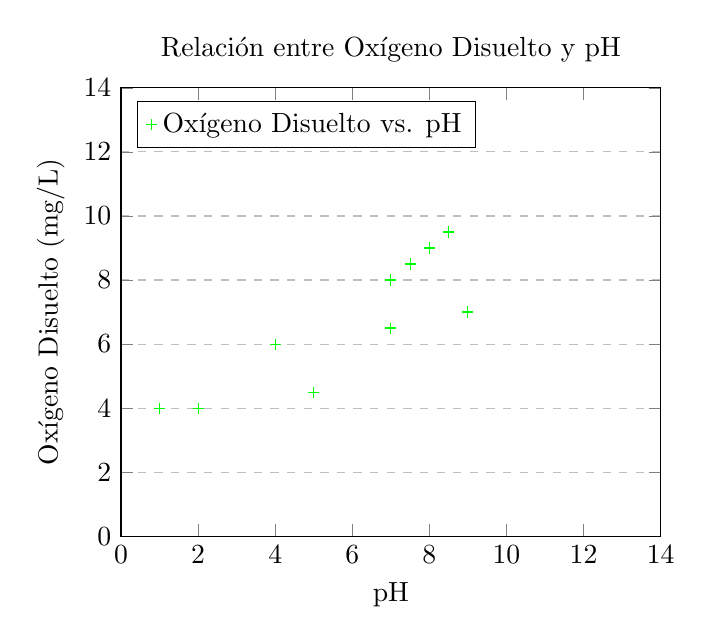
\begin{tikzpicture}
\begin{axis}[
    title={Relación entre Oxígeno Disuelto y pH},
    xlabel={pH},
    ylabel={Oxígeno Disuelto (mg/L)},
    xmin=0, xmax=14,
    ymin=0, ymax=14,
    xtick={0,2,...,14},
    ytick={0,2,...,14},
    legend pos=north west,
    ymajorgrids=true,
    grid style=dashed,
    scatter/classes={
        a={mark=+,draw=green}}
]
% Add your actual data points here
\addplot[scatter,only marks,scatter src=explicit symbolic]
table[meta=label] {
    x y label
    7 8 a
    8 9 a
    2 4 a
    1 4 a
    4 6 a
    5 4.5 a
    7 6.5 a
    9 7 a
    7.5 8.5 a
    8.5 9.5 a
    % More points...
};
\legend{Oxígeno Disuelto vs. pH}
\end{axis}
\end{tikzpicture}
\caption{Ejemplo de diagrama de dispersión entre Oxígeno Disuelto y pH}
\label{fig:distribucionNormal}
\end{figure}

\subsubsection{Covarianza}

La covarianza, similar a los momentos centrales univariados, se define como:
\[
\text{Cov}(X, Y) = \sigma_{xy} = \mathrm{E}\left\{ (X - m_x)(Y - m_y) \right\}
\]
y se calcula mediante:
\[
\sigma_{xy} = \frac{1}{N} \sum_{i=1}^{N} (x_i - m_x)(y_i - m_y)
\]

\subsubsection{Semivariograma}

El semivariograma mide la disimilaridad entre puntos con respecto a una línea de pendiente 45º, definido como:
\[
\gamma_{xy} = \frac{1}{2N} \sum_{i=1}^{N} \left( x_i - y_i \right)^2
\]

\subsubsection{Métodos de Correlación Estadística}

La correlación mide la relación lineal entre dos variables aleatorias. Se emplean tres métodos: Pearson, Spearman y Kendall, cada uno con sus propias aplicaciones.

\paragraph{Coeficiente de Correlación Lineal de Pearson}

El coeficiente de Pearson (\( r \)) mide la relación lineal entre dos variables cuantitativas:
\[
r = \frac{\sum (X_i - \bar{X})(Y_i - \bar{Y})}{\sqrt{\sum (X_i - \bar{X})^2 \sum (Y_i - \bar{Y})^2}}
\]

\paragraph{Coeficiente de Correlación de Rango de Spearman}

El coeficiente de Spearman (\( \rho \)) mide la correlación de rangos para datos ordinales:
\[
\rho = 1 - \frac{6 \sum d_i^2}{n(n^2 - 1)}
\]

\paragraph{Coeficiente de Correlación de Rango de Kendall}

El coeficiente de Kendall (\( \tau \)) mide la similitud de órdenes entre datos:
\[
\tau = \frac{2}{n(n-1)} \sum_{i<j} \text{sgn}(X_i - X_j) \text{sgn}(Y_i - Y_j)
\]

Estos métodos son herramientas clave para analizar relaciones entre variables en diversos campos de investigación.




\subsubsection{Regresión lineal}
La regresión lineal es una técnica estadística clave para comprender la relación entre variables, siendo útil en predicciones y pronósticos. Esta técnica busca describir la relación mediante una línea recta, cuyos parámetros se determinan generalmente utilizando el método de Mínimos Cuadrados. Este método minimiza la suma de los cuadrados de las diferencias entre los valores observados y los predichos, proporcionando la mejor aproximación posible. 

Existen varias formas de Mínimos Cuadrados, incluyendo:

\begin{itemize}[leftmargin=*]
  \item \textbf{Mínimos Cuadrados Ordinarios (MCO)}: Método básico y común.
  \item \textbf{Mínimos Cuadrados Ponderados (MCP)}: Asigna pesos diferentes a las observaciones.
  \item \textbf{Mínimos Cuadrados Generalizados (MCG)}: Para situaciones más complejas.
\end{itemize}

En un modelo lineal donde \( Y \) depende linealmente de \( X \) (\( Y = \beta_0 + \beta_1X + e \)), estos métodos determinan \( \beta_0 \) y \( \beta_1 \) minimizando la suma de los cuadrados de los residuos \( e \). Los residuos son las diferencias entre los valores observados de \( Y \) y los predichos por el modelo. 

Condiciones que deben cumplir los residuos:
\begin{itemize}
    \item \( \mathbb{E}\{e_i\} = 0 \) (valor esperado cero)
    \item \( \text{Var}\{e_i\} = \sigma_e^2 \) (varianza constante)
    \item \( \text{Cov}\{e_i, e_j\} = 0 \) para \( i \neq j \) (no correlacionados)
    \item \( e_i \sim \mathcal{N}(0, \sigma_e^2) \) (distribución normal)
\end{itemize}

\subsubsection{Mínimos Cuadrados Ordinarios (MCO)}
El objetivo de los MCO es encontrar los parámetros del modelo que minimicen la suma de los cuadrados de los errores:
\[ \text{SCR} = \sum_{i=1}^{N} (y_i - \hat{y}_i)^2 = \sum_{i=1}^{N} \left( y_i - (\hat{\beta}_0 + \hat{\beta}_1 x_i) \right)^2 \]
Resolviendo el sistema de ecuaciones:
\[ \frac{\partial \text{SCR}}{\partial \beta_0} = 0, \quad \frac{\partial \text{SCR}}{\partial \beta_1} = 0 \]

\subsection*{Coeficiente de determinación \( R^2 \)}
El coeficiente \( R^2 \) mide la bondad del ajuste del modelo lineal, representando la proporción de la varianza explicada por la regresión. Un \( R^2 \) cercano a 1 indica un buen ajuste, mientras que un \( R^2 \) cercano a 0 sugiere poca o ninguna relación lineal entre las variables.

\subsection*{Criterios de bondad del ajuste}
\begin{itemize}
    \item \( R^2 \approx 1 \) indica un buen ajuste lineal.
    \item \( R^2 \approx 0 \) sugiere que no hay una relación lineal significativa.
\end{itemize}

\subsection{Análisis variográfico de los datos}
El análisis variográfico es fundamental para evaluar cómo varían los valores de una variable aleatoria \( Z \) distribuidos en un dominio espacial \(\Omega\). Este análisis permite construir modelos geoestadísticos que describen la estructura espacial y la dependencia entre puntos en el espacio, facilitando así estimaciones más precisas de los valores no muestreados \cite{Viera2002}.



\subsection{Función aleatoria}

Una función aleatoria \(z(x)\) se define como una variable aleatoria regionalizada en una región \(\Omega\), representando un conjunto infinito de variables aleatorias en cada punto del dominio. Los valores regionalizados \(z(x_i)\) no pueden modelarse generalmente con una función determinista simple debido a su complejidad, por lo que se adopta un enfoque probabilístico considerando el mecanismo generador de datos como aleatorio. Un ejemplo de esto son los niveles de parámetros fisicoquímicos en la Laguna de Pacucha.

\subsubsection*{Variable Regionalizada}

Una \textbf{variable regionalizada} es una muestra de una función aleatoria en el espacio o tiempo, constituyendo una realización de la función aleatoria. Estas variables son esenciales en estudios geoestadísticos, como en la medición de oxígeno disuelto, temperatura y pH en diferentes puntos de un lago:

\begin{itemize}
    \item \textbf{Oxígeno Disuelto}: Indica la cantidad de oxígeno disponible en el agua.
    \item \textbf{Temperatura}: Influye en la solubilidad del oxígeno y la actividad biológica.
    \item \textbf{pH}: Refleja la acidez o alcalinidad del agua, afectando la disponibilidad de nutrientes.
\end{itemize}

\subsubsection{Función de distribución de una Función Aleatoria}

Para una función aleatoria \(Z(x)\) en una región \(\Omega\), el vector aleatorio
\[
\{ Z(x_1), Z(x_2), \ldots, Z(x_n) \}
\]
se caracteriza por su función de distribución de probabilidad \(n\)-variada:
\[
F_{Z(x_1),Z(x_2),\ldots,Z(x_n)}(z_1, z_2, \ldots, z_n) = \Pr\left( Z(x_1) \leq z_1, Z(x_2) \leq z_2, \ldots, Z(x_n) \leq z_n \right).
\]
Esta ley espacial de probabilidad es difícil de determinar completamente, por lo que usualmente se infieren los primeros momentos de la distribución.

\subsubsection{Momentos de una función aleatoria}

\paragraph{Momento de primer orden}
El primer momento, o valor medio \(m(\bar{x})\), se define como:
\[
m(\bar{x}) = \mathbb{E}[Z(\bar{x})],
\]
donde \(m\) depende de la posición \(x\).

\paragraph{Momento de segundo orden}
\textbf{Varianza} de \(Z(\bar{x})\):
\[
\sigma^2 = \text{Var}[Z] = \mathbb{E}[(Z - m)^2] \geq 0.
\]
\textbf{Covarianza} entre \(Z(x_i)\) y \(Z(x_j)\):
\[
Z(\bar{x}_i, \bar{x}_j) = \mathbb{E}\left[\{z(\bar{x}_i) - m(\bar{x}_i)\} \{z(\bar{x}_j) - m(\bar{x}_j)\}\right].
\]
\textbf{Semivariograma} de \(Z(\bar{x})\):
\[
\gamma(x_i, x_j) = \frac{1}{2} \mathbb{E} \left[ \left( Z(x_i) - Z(x_j) \right)^2 \right].
\]

\subsection{Funciones aleatorias estacionarias}

Una función aleatoria es estacionaria si su función de distribución permanece constante ante cualquier traslación en relación con un vector \(h\). Esto implica que los momentos de primer y segundo orden no varían con las traslaciones:
\[
\mathbb{E}[Z(\bar{x})] = m, \quad \text{Var}[Z(\bar{x})] = \sigma^2, \quad C(\bar{h}) = \mathbb{E} [Z(\bar{x}+\bar{h})Z(\bar{x})] - m^2.
\]

\subsection{Funciones aleatorias intrínsecas}

Las funciones aleatorias intrínsecas cumplen con las siguientes condiciones:

\begin{itemize}
    \item \( \mathbb{E}[Z(\bar{x}+\bar{h})-Z(\bar{x})] = k \) (valor esperado de las diferencias es constante)
    \item \( \text{Var}[Z(\bar{x}+\bar{h})-Z(\bar{x})] = 2\gamma(\bar{h}) \) (varianza de las diferencias)
\end{itemize}

Estas condiciones forman la \textit{Hipótesis Intrínseca}. Una función estacionaria de segundo orden es intrínseca, pero no todas las funciones intrínsecas son estacionarias de segundo orden.

\subsection{Funciones aleatorias no estacionarias}

Estas funciones no satisfacen la \textit{hipótesis intrínseca}, con un valor esperado y varianza de las diferencias que varían según la posición. El variograma puede indicar la no estacionariedad cuando muestra un crecimiento mayor o igual a \(h^2\).

\subsection{Análisis estructural del variograma}

El análisis variográfico estudia la consistencia espacial de una característica. Para construir el variograma experimental, se toman muestras en ubicaciones conocidas, y se ajusta un modelo teórico para prever el patrón espacial de la característica. La elección del modelo de variograma válido es crucial para lograr predicciones precisas mediante interpolaciones de kriging \cite{Mahdi2020}.


\section{Análisis variográfico }

Consiste en construir una función que representa la correlación espacial de los datos muestreados y la relación de dependencia a partir de ciertos supuestos de estacionariedad.
\section{	Semivariograma}

El \textbf{semivariograma}, conocido también como variograma, es la herramienta central de la geoestadística. Dada una FA \( Z(x) \) que cumpla la Hipótesis Intrínseca entonces existe la función semivarianza y se define como sigue:

\[
\gamma(h) = \frac{1}{2} \text{Var} [Z(x) - Z(x+h)] = \frac{1}{2} E \left[ \left( Z(x) - Z(x+h) \right)^2 \right]
\]

En general, este variograma \( 2\gamma(x,h) \) es una función tanto del punto \( x \) como del vector \( h \). Por lo tanto, la estimación de este variograma requiere varias realizaciones, \([z_k (x),z_k (x+h)]\), \([z_{k'} (x),z_{k'} (x+h)]\), \(\ldots [z_{k''} (x),z_{k''} (x+h)]\) de la pareja de variables aleatorias \([Z(x)-Z(x-h)]\). Ahora bien, en la práctica, al menos en las aplicaciones para estimar concentraciones de contaminantes o parámetros fisicoquímicas, solo existe una realización de este tipo \([Z(x)-Z(x-h)]\). Para solucionar este problema, se introduce la \textit{hipótesis intrínseca}. Esta hipótesis es que la función variograma \( 2\gamma(x,h) \) depende solo del vector de separación \( h \) (módulo y dirección) y no de la ubicación \( x \). Entonces es posible estimar el variograma \( 2\gamma(x,h) \) a partir de los datos disponibles: un estimador \( 2\gamma^*(h) \) es la media aritmética de las diferencias cuadradas entre dos medidas experimentales \([Z(x_i )-Z(x_i-h)]\) en dos puntos separados por el vector \( h \); es decir:
\[
\tilde{\gamma}(h) = \frac{1}{2N(h)} \sum_{i=1}^{N(h)} [Z(x_i-h)-Z(x_i)]^2
\]
\subsection{	Variograma teórico y experimental}

\subsubsection*{Variograma Teórico}

El variograma teórico es un modelo matemático que representa la variabilidad espacial esperada en un conjunto de datos geoespaciales. Este modelo se ajusta a los datos experimentales para describir cómo la correlación espacial debería comportarse idealmente. Se utiliza para predecir cómo se deberían comportar las semivarianzas a diferentes distancias si los datos siguieran un patrón específico de correlación espacial.

Los variogramas teóricos generalmente se describen con tres parámetros principales:
\begin{description}[leftmargin=1cm, style=sameline]
    \item[Nugget (Efecto Pepita):] La variabilidad a una escala menor que la mínima distancia entre puntos de muestreo.
    \item[Sill (Meseta):] La variabilidad total que se alcanza a medida que la distancia entre los puntos de muestreo aumenta.
    \item[Rango:] La distancia a la cual la variabilidad alcanza el sill y se estabiliza.
\end{description}

\subsubsection*{Variograma Experimental}

El variograma experimental se calcula directamente a partir de los datos observados. Es una medida empírica de cómo varía la diferencia entre los valores de las observaciones a medida que aumenta la distancia entre las ubicaciones. En otras palabras, representa la estructura real de correlación espacial presente en los datos observados.

Se utiliza para determinar los parámetros del variograma teórico (nugget, sill y rango) ajustando un modelo teórico a los datos experimentales. Este modelo ajustado se utiliza luego en técnicas como el kriging para realizar interpolación espacial precisa y en simulaciones estocásticas para analizar la incertidumbre espacial.
\section{Modelos de Variogramas}

A continuación, se describen algunos modelos comunes de variogramas con sus respectivas fórmulas en una tabla comparativa.


\subsection{Modelo Esférico}

La fórmula para el modelo esférico es la siguiente:
\[
\gamma(h) =
\begin{cases}
\frac{S}{2} \left( \frac{3(h/a)}{2} - \left(\frac{h/a}{3}\right)^3 \right) & \text{para } 0 \leq h \leq a, \\
S & \text{para } h > a.
\end{cases}
\]

\begin{figure}[h!]
\centering
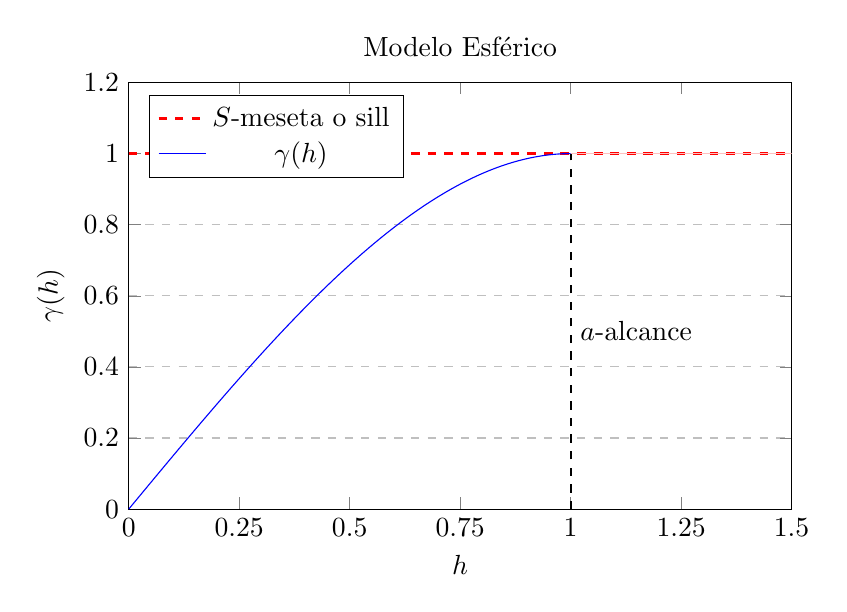
\begin{tikzpicture}
\begin{axis}[
    title={Modelo Esférico},
    xlabel={$h$},
    ylabel={$\gamma(h)$},
    xmin=0, xmax=1.5,
    ymin=0, ymax=1.2,
    xtick={0,0.25,0.5,0.75,1,1.25,1.5},
    ytick={0,0.2,0.4,0.6,0.8,1,1.2},
    legend pos=north west,
    ymajorgrids=true,
    grid style=dashed,
    width=10cm,
    height=7cm
]

% Sill
\addplot[
    color=red,
    mark=none,
    domain=0:1.5,
    samples=200,
    thick,
    dashed
    ]
    {1};
\addlegendentry{$S$-meseta o sill}

% Modelo Esférico
\addplot[
    color=blue,
    mark=none,
    domain=0:1,
    samples=200,
    ]
    {(3*x/2 - (x^3)/2)};
\addplot[
    color=pink,
    mark=none,
    domain=1:1.5,
    samples=200,
    ]
    {1};
\addlegendentry{$\gamma(h)$}

% Range
\draw [dashed, thick] (axis cs:1,0) -- (axis cs:1,1);
\node[anchor=west] at (axis cs:1,0.5) {$a$-alcance};

\end{axis}
\end{tikzpicture}
\caption{Modelo Esférico de variograma}
\end{figure}


\subsection{Modelo Exponencial}

La fórmula para el modelo exponencial es la siguiente:
\[
\gamma(h) = S \left[ 1 - \exp\left(-\frac{3h}{a}\right) \right] \text{ para } h \geq 0
\]

\begin{figure}[h!]
\centering
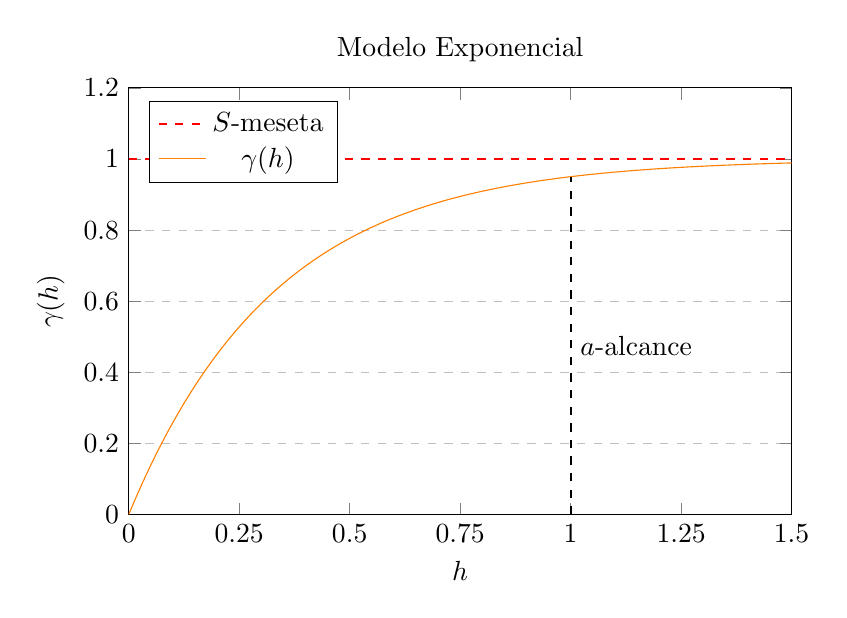
\begin{tikzpicture}
\begin{axis}[
    title={Modelo Exponencial},
    xlabel={$h$},
    ylabel={$\gamma(h)$},
    xmin=0, xmax=1.5,
    ymin=0, ymax=1.2,
    xtick={0,0.25,0.5,0.75,1,1.25,1.5},
    ytick={0,0.2,0.4,0.6,0.8,1,1.2},
    legend pos=north west,
    ymajorgrids=true,
    grid style=dashed,
    width=10cm,
    height=7cm
]

% Sill
\addplot[
    color=red,
    mark=none,
    domain=0:1.5,
    samples=200,
    thick,
    dashed
    ]
    {1};
\addlegendentry{$S$-meseta}

% Modelo Exponencial
\addplot[
    color=orange,
    mark=none,
    domain=0:1.5,
    samples=200,
    ]
    {1 - exp(-3*x)};
\addlegendentry{$\gamma(h)$}

% Range
\draw [dashed, thick] (axis cs:1,0) -- (axis cs:1,{1 - exp(-3)});
\node[anchor=west] at (axis cs:1,{(1 - exp(-3))/2}) {$a$-alcance};

\end{axis}
\end{tikzpicture}
\caption{Modelo Exponencial de variograma}
\end{figure}


\subsection{Modelo Gaussiano}

La fórmula para el modelo gaussiano es la siguiente:
\[
\gamma(h) = S \left[ 1 - \exp\left(-\left(\frac{3h}{a}\right)^2\right) \right] \text{ para } h \geq 0
\]

\begin{figure}[h!]
\centering
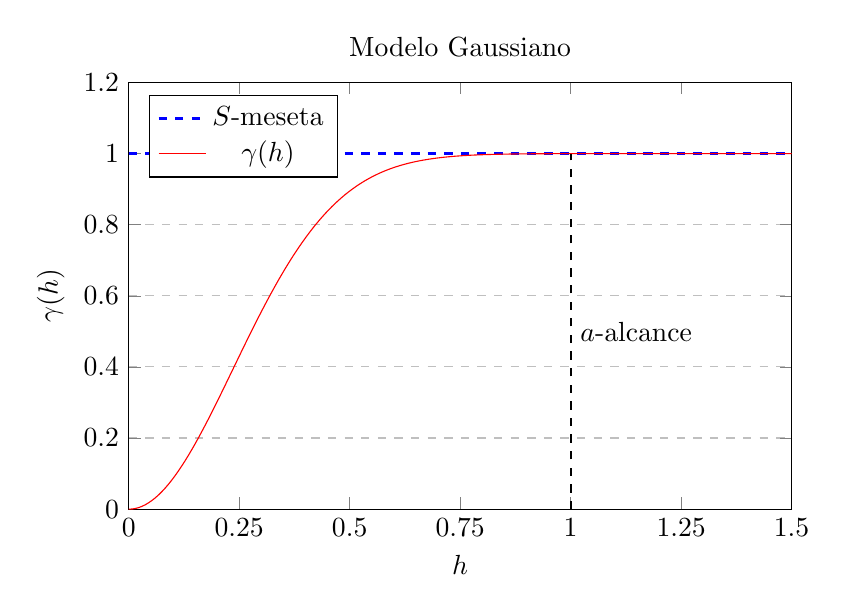
\begin{tikzpicture}
\begin{axis}[
    title={Modelo Gaussiano},
    xlabel={$h$},
    ylabel={$\gamma(h)$},
    xmin=0, xmax=1.5,
    ymin=0, ymax=1.2,
    xtick={0,0.25,0.5,0.75,1,1.25,1.5},
    ytick={0,0.2,0.4,0.6,0.8,1,1.2},
    legend pos=north west,
    ymajorgrids=true,
    grid style=dashed,
    width=10cm,
    height=7cm
]

% Sill
\addplot[
    color=blue,
    mark=none,
    domain=0:1.5,
    samples=200,
    thick,
    dashed
    ]
    {1};
\addlegendentry{$S$-meseta}

% Modelo Gaussiano
\addplot[
    color=red,
    mark=none,
    domain=0:1.5,
    samples=200,
    ]
    {1 - exp(-(3*x)^2)};
\addlegendentry{$\gamma(h)$}

% Range
\draw [dashed, thick] (axis cs:1,0) -- (axis cs:1,{1 - exp(-9)});
\node[anchor=west] at (axis cs:1,{(1 - exp(-9))/2}) {$a$-alcance};

\end{axis}
\end{tikzpicture}
\caption{Modelo Gaussiano de variograma}
\end{figure}

\section{Predicciones}


La realización de una interpolación posibilita la estimación, permitiendo mapear con precisión el fenómeno de contaminación. Esto ofrece una visualización detallada de la distribución del contaminante en el área estudiada. El método más conocido es el método del \textbf{Kriging} o \textbf{Krigeado}.

\subsection{Kriging}

El Kriging es un método de interpolación y estimación utilizado en estadística espacial para predecir valores en ubicaciones no muestreadas a partir de datos observados en ubicaciones conocidas.

En los alrededores de 1960, se acuñó el término ``krigeado'' para referirse a una técnica desarrollada en Francia por Matheron, basada en los trabajos de D. G. Krige. Krige fue posiblemente el primero en utilizar la correlación espacial y el mejor estimador lineal no sesgado en la evaluación de yacimientos minerales. El krigeado, por definición, es un método de estimación lineal sin sesgo que tiene como objetivo minimizar la variabilidad en las estimaciones. Esta técnica se utiliza para predecir los valores de una variable en ubicaciones donde no se disponen de datos, utilizando la información de los valores en puntos cercanos.


\subsubsection*{Descripción de las Propiedades del Estimador \( Z_0^* \)}

\begin{itemize}
  \item \textbf{Estimador:} Se refiere a una regla o método para calcular una estimación de una cantidad desconocida a partir de datos observados. En este caso, \( Z_0^* \) representa el estimador.
  \[
  Z_0^*
  \]

  \item \textbf{Mejor:} En el contexto de los estimadores, "mejor" se refiere a aquel que tiene menor varianza entre todos los estimadores insesgados, conocido como el estimador de mínima varianza insesgado . Aquí se busca minimizar la varianza del error del estimador \( Z_0^* \) respecto al parámetro verdadero \( Z_0 \).
  \[
  \min \left\{ \text{Var} \left[ Z_0 - Z_0^* \right] \right\}
  \]

  \item \textbf{Lineal:} Indica que el estimador \( Z_0^* \) es una combinación lineal de las variables observadas \( Z_i \), donde \( \lambda_i \) son los pesos asignados a cada observación.
  \[
  Z_0^* = \sum_{i=1}^{N} \lambda_i Z_i
  \]

  \item \textbf{Insesgado:} Un estimador es insesgado si su valor esperado es igual al verdadero valor del parámetro que se estima. Esto significa que, en promedio, el estimador acierta el parámetro verdadero.
  
  \[
  E\left[Z_0^*\right] = E\left[Z_0\right]
  \]
  
\end{itemize}


\subsection{Kriging Lineal}

El kriging es una técnica esencial en geoestadística para la estimación espacial, basada en la teoría de variables aleatorias regionalizadas. A continuación, se describen las variantes más comunes del kriging lineal, con un énfasis especial en el kriging ordinario debido a su relevancia en este estudio.

\begin{itemize}
    \item \textbf{Kriging Simple}: Esta variante supone un promedio global conocido \(\mu\) para la estimación en una región no muestreada. La estimación \(Z^*(\mathbf{x}_0)\) en la ubicación \(\mathbf{x}_0\) se obtiene ajustando los pesos \(\lambda_i\) de las observaciones \(Z(\mathbf{x}_i)\) para minimizar la varianza del error, con la condición de que la suma de los pesos sea 1 \cite{Viera2002}.
    \[
    Z^*(\mathbf{x}_0) = \mu + \sum_{i=1}^{n} \lambda_i (Z(\mathbf{x}_i) - \mu)
    \]
    
    \item \textbf{Kriging Ordinario}: A diferencia del kriging simple, el kriging ordinario no requiere conocer el promedio \(\mu\). En su lugar, estima implícitamente el promedio a partir de los datos disponibles, lo que lo hace más adaptable a variaciones locales. La estimación \(Z^*(\mathbf{x}_0)\) se expresa como una combinación ponderada de las observaciones:
    \[
    Z^*(\mathbf{x}_0) = \sum_{i=1}^{n} \lambda_i Z(\mathbf{x}_i)
    \]
    El kriging ordinario es particularmente eficaz en situaciones donde la media no es constante o se desconoce, proporcionando estimaciones robustas y precisas incluso en presencia de heterogeneidad espacial \cite{Viera2002}.
    
    \item \textbf{Kriging Universal}: Este método extiende el kriging ordinario incorporando una función de tendencia \(f_i(\mathbf{x})\) con coeficientes desconocidos \(\beta_i\). Es adecuado cuando los datos muestran una tendencia que puede modelarse, como un polinomio:
    \[
    Z^*(\mathbf{x}_0) = \sum_{i=1}^{m} \beta_i f_i(\mathbf{x}) + \sum_{i=1}^{n} \lambda_i Z(\mathbf{x}_i)
    \]
    
    \item \textbf{Kriging Residual}: Este enfoque se utiliza cuando los datos pueden descomponerse en una tendencia conocida \(\hat{m}(\mathbf{x}_0)\) y residuos estocásticos. Primero se modela y sustrae la tendencia de los datos, y luego se aplica kriging a los residuos:
    \[
    Z^*(\mathbf{x}_0) = \hat{m}(\mathbf{x}_0) + \sum_{i=1}^{n} \lambda_i (Z(\mathbf{x}_i) - \hat{m}(\mathbf{x}_i))
    \]
\end{itemize}

\subsection{Kriging No Lineal}

El kriging no lineal incluye métodos que son útiles cuando las relaciones entre las variables no son lineales.

\begin{itemize}
    \item \textbf{Kriging Disyuntivo}: Modela la distribución de probabilidad condicional de los datos transformados a una escala normal, útil para relaciones no lineales.
    \[
    Z^*(\mathbf{x}_0) = F^{-1}\left(\sum \lambda_i F(Z(\mathbf{x}_i))\right)
    \]
    
    \item \textbf{Kriging Indicador}: Estima la probabilidad de que una variable aleatoria exceda ciertos umbrales, modelando la incertidumbre y la probabilidad de eventos específicos.
    \[
    I^*(\mathbf{x}_0) = \sum_{i=1}^{n} \lambda_i I(\mathbf{x}_i)
    \]
    
    \item \textbf{Kriging Probabilístico}: Estima la probabilidad de que una variable exceda un umbral \(z\), útil en geología y minería.
    \[
    P^*(\mathbf{x}_0) = \sum_{i=1}^{n} \lambda_i P(Z(\mathbf{x}_i) > z)
    \]
\end{itemize}

\subsection{Según el Soporte de la Medición de los Datos}

\begin{itemize}
    \item \textbf{Puntual}: Estimaciones para puntos específicos.
    \item \textbf{En Bloques}: Estimaciones para áreas o volúmenes más grandes.
\end{itemize}

\subsection{Kriging Paramétrico y No Paramétrico}

\begin{itemize}
    \item \textbf{Paramétrico}: Supone un modelo paramétrico específico.
    \item \textbf{No Paramétrico}: No hace suposiciones sobre la forma del modelo.
    \end{itemize}

\section{Verificación de Matrices Semidefinidas Positivas en Coregionalización}

El análisis multivariado en geoestadística, especialmente mediante modelos de coregionalización, es fundamental para entender la interdependencia entre múltiples variables espaciales. A diferencia del enfoque univariado, permite modelar conjuntamente dos o más variables aleatorias, mejorando la estimación espacial al considerar la correlación cruzada.

Una matriz \(\mathbf{L}\) es semidefinida positiva si para todo vector no nulo \(b \in \mathbb{R}^n\), se cumple que \(b'\mathbf{L}b \geq 0\). Verificar esta propiedad es esencial en los modelos de coregionalización para asegurar varianzas no negativas. Consideremos una matriz de coregionalización \(\mathbf{L}\) dada por:

\[
\mathbf{L} = 
\begin{bmatrix}
l_{11} & l_{12} \\
l_{21} & l_{22}
\end{bmatrix}
\]

Para que \(\mathbf{L}\) sea semidefinida positiva, debe cumplir dos condiciones:
\begin{enumerate}
    \item Los elementos de la diagonal principal deben ser no negativos: \(l_{11} \geq 0\) y \(l_{22} \geq 0\).
    \item El determinante de \(\mathbf{L}\) debe ser no negativo:
    \[
    \det(\mathbf{L}) = l_{11}l_{22} - l_{12}l_{21} \geq 0
    \]
    Esto asegura que la matriz no tiene valores propios negativos.
\end{enumerate}

Cumpliendo estas condiciones, podemos afirmar que \(\mathbf{L}\) es semidefinida positiva y adecuada para su uso en modelos de coregionalización lineal.
